\documentclass[11pt]{article}

    \usepackage[breakable]{tcolorbox}
    \usepackage{parskip} % Stop auto-indenting (to mimic markdown behaviour)
    \usepackage{ctex}

    % Basic figure setup, for now with no caption control since it's done
    % automatically by Pandoc (which extracts ![](path) syntax from Markdown).
    \usepackage{graphicx}
    % Maintain compatibility with old templates. Remove in nbconvert 6.0
    \let\Oldincludegraphics\includegraphics
    % Ensure that by default, figures have no caption (until we provide a
    % proper Figure object with a Caption API and a way to capture that
    % in the conversion process - todo).
    \usepackage{caption}
    \DeclareCaptionFormat{nocaption}{}
    \captionsetup{format=nocaption,aboveskip=0pt,belowskip=0pt}

    \usepackage{float}
    \floatplacement{figure}{H} % forces figures to be placed at the correct location
    \usepackage{xcolor} % Allow colors to be defined
    \usepackage{enumerate} % Needed for markdown enumerations to work
    \usepackage{geometry} % Used to adjust the document margins
    \usepackage{amsmath} % Equations
    \usepackage{amssymb} % Equations
    \usepackage{textcomp} % defines textquotesingle
    % Hack from http://tex.stackexchange.com/a/47451/13684:
    \AtBeginDocument{%
        \def\PYZsq{\textquotesingle}% Upright quotes in Pygmentized code
    }
    \usepackage{upquote} % Upright quotes for verbatim code
    \usepackage{eurosym} % defines \euro

    \usepackage{iftex}
    \ifPDFTeX
        \usepackage[T1]{fontenc}
        \IfFileExists{alphabeta.sty}{
              \usepackage{alphabeta}
          }{
              \usepackage[mathletters]{ucs}
              \usepackage[utf8x]{inputenc}
          }
    \else
        \usepackage{fontspec}
        \usepackage{unicode-math}
    \fi

    \usepackage{fancyvrb} % verbatim replacement that allows latex
    \usepackage{grffile} % extends the file name processing of package graphics
                         % to support a larger range
    \makeatletter % fix for old versions of grffile with XeLaTeX
    \@ifpackagelater{grffile}{2019/11/01}
    {
      % Do nothing on new versions
    }
    {
      \def\Gread@@xetex#1{%
        \IfFileExists{"\Gin@base".bb}%
        {\Gread@eps{\Gin@base.bb}}%
        {\Gread@@xetex@aux#1}%
      }
    }
    \makeatother
    \usepackage[Export]{adjustbox} % Used to constrain images to a maximum size
    \adjustboxset{max size={0.9\linewidth}{0.9\paperheight}}

    % The hyperref package gives us a pdf with properly built
    % internal navigation ('pdf bookmarks' for the table of contents,
    % internal cross-reference links, web links for URLs, etc.)
    \usepackage{hyperref}
    % The default LaTeX title has an obnoxious amount of whitespace. By default,
    % titling removes some of it. It also provides customization options.
    \usepackage{titling}
    \usepackage{longtable} % longtable support required by pandoc >1.10
    \usepackage{booktabs}  % table support for pandoc > 1.12.2
    \usepackage{array}     % table support for pandoc >= 2.11.3
    \usepackage{calc}      % table minipage width calculation for pandoc >= 2.11.1
    \usepackage[inline]{enumitem} % IRkernel/repr support (it uses the enumerate* environment)
    \usepackage[normalem]{ulem} % ulem is needed to support strikethroughs (\sout)
                                % normalem makes italics be italics, not underlines
    \usepackage{mathrsfs}
    

    
    % Colors for the hyperref package
    \definecolor{urlcolor}{rgb}{0,.145,.698}
    \definecolor{linkcolor}{rgb}{.71,0.21,0.01}
    \definecolor{citecolor}{rgb}{.12,.54,.11}

    % ANSI colors
    \definecolor{ansi-black}{HTML}{3E424D}
    \definecolor{ansi-black-intense}{HTML}{282C36}
    \definecolor{ansi-red}{HTML}{E75C58}
    \definecolor{ansi-red-intense}{HTML}{B22B31}
    \definecolor{ansi-green}{HTML}{00A250}
    \definecolor{ansi-green-intense}{HTML}{007427}
    \definecolor{ansi-yellow}{HTML}{DDB62B}
    \definecolor{ansi-yellow-intense}{HTML}{B27D12}
    \definecolor{ansi-blue}{HTML}{208FFB}
    \definecolor{ansi-blue-intense}{HTML}{0065CA}
    \definecolor{ansi-magenta}{HTML}{D160C4}
    \definecolor{ansi-magenta-intense}{HTML}{A03196}
    \definecolor{ansi-cyan}{HTML}{60C6C8}
    \definecolor{ansi-cyan-intense}{HTML}{258F8F}
    \definecolor{ansi-white}{HTML}{C5C1B4}
    \definecolor{ansi-white-intense}{HTML}{A1A6B2}
    \definecolor{ansi-default-inverse-fg}{HTML}{FFFFFF}
    \definecolor{ansi-default-inverse-bg}{HTML}{000000}

    % common color for the border for error outputs.
    \definecolor{outerrorbackground}{HTML}{FFDFDF}

    % commands and environments needed by pandoc snippets
    % extracted from the output of `pandoc -s`
    \providecommand{\tightlist}{%
      \setlength{\itemsep}{0pt}\setlength{\parskip}{0pt}}
    \DefineVerbatimEnvironment{Highlighting}{Verbatim}{commandchars=\\\{\}}
    % Add ',fontsize=\small' for more characters per line
    \newenvironment{Shaded}{}{}
    \newcommand{\KeywordTok}[1]{\textcolor[rgb]{0.00,0.44,0.13}{\textbf{{#1}}}}
    \newcommand{\DataTypeTok}[1]{\textcolor[rgb]{0.56,0.13,0.00}{{#1}}}
    \newcommand{\DecValTok}[1]{\textcolor[rgb]{0.25,0.63,0.44}{{#1}}}
    \newcommand{\BaseNTok}[1]{\textcolor[rgb]{0.25,0.63,0.44}{{#1}}}
    \newcommand{\FloatTok}[1]{\textcolor[rgb]{0.25,0.63,0.44}{{#1}}}
    \newcommand{\CharTok}[1]{\textcolor[rgb]{0.25,0.44,0.63}{{#1}}}
    \newcommand{\StringTok}[1]{\textcolor[rgb]{0.25,0.44,0.63}{{#1}}}
    \newcommand{\CommentTok}[1]{\textcolor[rgb]{0.38,0.63,0.69}{\textit{{#1}}}}
    \newcommand{\OtherTok}[1]{\textcolor[rgb]{0.00,0.44,0.13}{{#1}}}
    \newcommand{\AlertTok}[1]{\textcolor[rgb]{1.00,0.00,0.00}{\textbf{{#1}}}}
    \newcommand{\FunctionTok}[1]{\textcolor[rgb]{0.02,0.16,0.49}{{#1}}}
    \newcommand{\RegionMarkerTok}[1]{{#1}}
    \newcommand{\ErrorTok}[1]{\textcolor[rgb]{1.00,0.00,0.00}{\textbf{{#1}}}}
    \newcommand{\NormalTok}[1]{{#1}}

    % Additional commands for more recent versions of Pandoc
    \newcommand{\ConstantTok}[1]{\textcolor[rgb]{0.53,0.00,0.00}{{#1}}}
    \newcommand{\SpecialCharTok}[1]{\textcolor[rgb]{0.25,0.44,0.63}{{#1}}}
    \newcommand{\VerbatimStringTok}[1]{\textcolor[rgb]{0.25,0.44,0.63}{{#1}}}
    \newcommand{\SpecialStringTok}[1]{\textcolor[rgb]{0.73,0.40,0.53}{{#1}}}
    \newcommand{\ImportTok}[1]{{#1}}
    \newcommand{\DocumentationTok}[1]{\textcolor[rgb]{0.73,0.13,0.13}{\textit{{#1}}}}
    \newcommand{\AnnotationTok}[1]{\textcolor[rgb]{0.38,0.63,0.69}{\textbf{\textit{{#1}}}}}
    \newcommand{\CommentVarTok}[1]{\textcolor[rgb]{0.38,0.63,0.69}{\textbf{\textit{{#1}}}}}
    \newcommand{\VariableTok}[1]{\textcolor[rgb]{0.10,0.09,0.49}{{#1}}}
    \newcommand{\ControlFlowTok}[1]{\textcolor[rgb]{0.00,0.44,0.13}{\textbf{{#1}}}}
    \newcommand{\OperatorTok}[1]{\textcolor[rgb]{0.40,0.40,0.40}{{#1}}}
    \newcommand{\BuiltInTok}[1]{{#1}}
    \newcommand{\ExtensionTok}[1]{{#1}}
    \newcommand{\PreprocessorTok}[1]{\textcolor[rgb]{0.74,0.48,0.00}{{#1}}}
    \newcommand{\AttributeTok}[1]{\textcolor[rgb]{0.49,0.56,0.16}{{#1}}}
    \newcommand{\InformationTok}[1]{\textcolor[rgb]{0.38,0.63,0.69}{\textbf{\textit{{#1}}}}}
    \newcommand{\WarningTok}[1]{\textcolor[rgb]{0.38,0.63,0.69}{\textbf{\textit{{#1}}}}}


    % Define a nice break command that doesn't care if a line doesn't already
    % exist.
    \def\br{\hspace*{\fill} \\* }
    % Math Jax compatibility definitions
    \def\gt{>}
    \def\lt{<}
    \let\Oldtex\TeX
    \let\Oldlatex\LaTeX
    \renewcommand{\TeX}{\textrm{\Oldtex}}
    \renewcommand{\LaTeX}{\textrm{\Oldlatex}}
    % Document parameters
    % Document title
    \title{实验二 排序算法}
    
    
    
    
    
% Pygments definitions
\makeatletter
\def\PY@reset{\let\PY@it=\relax \let\PY@bf=\relax%
    \let\PY@ul=\relax \let\PY@tc=\relax%
    \let\PY@bc=\relax \let\PY@ff=\relax}
\def\PY@tok#1{\csname PY@tok@#1\endcsname}
\def\PY@toks#1+{\ifx\relax#1\empty\else%
    \PY@tok{#1}\expandafter\PY@toks\fi}
\def\PY@do#1{\PY@bc{\PY@tc{\PY@ul{%
    \PY@it{\PY@bf{\PY@ff{#1}}}}}}}
\def\PY#1#2{\PY@reset\PY@toks#1+\relax+\PY@do{#2}}

\@namedef{PY@tok@w}{\def\PY@tc##1{\textcolor[rgb]{0.73,0.73,0.73}{##1}}}
\@namedef{PY@tok@c}{\let\PY@it=\textit\def\PY@tc##1{\textcolor[rgb]{0.24,0.48,0.48}{##1}}}
\@namedef{PY@tok@cp}{\def\PY@tc##1{\textcolor[rgb]{0.61,0.40,0.00}{##1}}}
\@namedef{PY@tok@k}{\let\PY@bf=\textbf\def\PY@tc##1{\textcolor[rgb]{0.00,0.50,0.00}{##1}}}
\@namedef{PY@tok@kp}{\def\PY@tc##1{\textcolor[rgb]{0.00,0.50,0.00}{##1}}}
\@namedef{PY@tok@kt}{\def\PY@tc##1{\textcolor[rgb]{0.69,0.00,0.25}{##1}}}
\@namedef{PY@tok@o}{\def\PY@tc##1{\textcolor[rgb]{0.40,0.40,0.40}{##1}}}
\@namedef{PY@tok@ow}{\let\PY@bf=\textbf\def\PY@tc##1{\textcolor[rgb]{0.67,0.13,1.00}{##1}}}
\@namedef{PY@tok@nb}{\def\PY@tc##1{\textcolor[rgb]{0.00,0.50,0.00}{##1}}}
\@namedef{PY@tok@nf}{\def\PY@tc##1{\textcolor[rgb]{0.00,0.00,1.00}{##1}}}
\@namedef{PY@tok@nc}{\let\PY@bf=\textbf\def\PY@tc##1{\textcolor[rgb]{0.00,0.00,1.00}{##1}}}
\@namedef{PY@tok@nn}{\let\PY@bf=\textbf\def\PY@tc##1{\textcolor[rgb]{0.00,0.00,1.00}{##1}}}
\@namedef{PY@tok@ne}{\let\PY@bf=\textbf\def\PY@tc##1{\textcolor[rgb]{0.80,0.25,0.22}{##1}}}
\@namedef{PY@tok@nv}{\def\PY@tc##1{\textcolor[rgb]{0.10,0.09,0.49}{##1}}}
\@namedef{PY@tok@no}{\def\PY@tc##1{\textcolor[rgb]{0.53,0.00,0.00}{##1}}}
\@namedef{PY@tok@nl}{\def\PY@tc##1{\textcolor[rgb]{0.46,0.46,0.00}{##1}}}
\@namedef{PY@tok@ni}{\let\PY@bf=\textbf\def\PY@tc##1{\textcolor[rgb]{0.44,0.44,0.44}{##1}}}
\@namedef{PY@tok@na}{\def\PY@tc##1{\textcolor[rgb]{0.41,0.47,0.13}{##1}}}
\@namedef{PY@tok@nt}{\let\PY@bf=\textbf\def\PY@tc##1{\textcolor[rgb]{0.00,0.50,0.00}{##1}}}
\@namedef{PY@tok@nd}{\def\PY@tc##1{\textcolor[rgb]{0.67,0.13,1.00}{##1}}}
\@namedef{PY@tok@s}{\def\PY@tc##1{\textcolor[rgb]{0.73,0.13,0.13}{##1}}}
\@namedef{PY@tok@sd}{\let\PY@it=\textit\def\PY@tc##1{\textcolor[rgb]{0.73,0.13,0.13}{##1}}}
\@namedef{PY@tok@si}{\let\PY@bf=\textbf\def\PY@tc##1{\textcolor[rgb]{0.64,0.35,0.47}{##1}}}
\@namedef{PY@tok@se}{\let\PY@bf=\textbf\def\PY@tc##1{\textcolor[rgb]{0.67,0.36,0.12}{##1}}}
\@namedef{PY@tok@sr}{\def\PY@tc##1{\textcolor[rgb]{0.64,0.35,0.47}{##1}}}
\@namedef{PY@tok@ss}{\def\PY@tc##1{\textcolor[rgb]{0.10,0.09,0.49}{##1}}}
\@namedef{PY@tok@sx}{\def\PY@tc##1{\textcolor[rgb]{0.00,0.50,0.00}{##1}}}
\@namedef{PY@tok@m}{\def\PY@tc##1{\textcolor[rgb]{0.40,0.40,0.40}{##1}}}
\@namedef{PY@tok@gh}{\let\PY@bf=\textbf\def\PY@tc##1{\textcolor[rgb]{0.00,0.00,0.50}{##1}}}
\@namedef{PY@tok@gu}{\let\PY@bf=\textbf\def\PY@tc##1{\textcolor[rgb]{0.50,0.00,0.50}{##1}}}
\@namedef{PY@tok@gd}{\def\PY@tc##1{\textcolor[rgb]{0.63,0.00,0.00}{##1}}}
\@namedef{PY@tok@gi}{\def\PY@tc##1{\textcolor[rgb]{0.00,0.52,0.00}{##1}}}
\@namedef{PY@tok@gr}{\def\PY@tc##1{\textcolor[rgb]{0.89,0.00,0.00}{##1}}}
\@namedef{PY@tok@ge}{\let\PY@it=\textit}
\@namedef{PY@tok@gs}{\let\PY@bf=\textbf}
\@namedef{PY@tok@gp}{\let\PY@bf=\textbf\def\PY@tc##1{\textcolor[rgb]{0.00,0.00,0.50}{##1}}}
\@namedef{PY@tok@go}{\def\PY@tc##1{\textcolor[rgb]{0.44,0.44,0.44}{##1}}}
\@namedef{PY@tok@gt}{\def\PY@tc##1{\textcolor[rgb]{0.00,0.27,0.87}{##1}}}
\@namedef{PY@tok@err}{\def\PY@bc##1{{\setlength{\fboxsep}{\string -\fboxrule}\fcolorbox[rgb]{1.00,0.00,0.00}{1,1,1}{\strut ##1}}}}
\@namedef{PY@tok@kc}{\let\PY@bf=\textbf\def\PY@tc##1{\textcolor[rgb]{0.00,0.50,0.00}{##1}}}
\@namedef{PY@tok@kd}{\let\PY@bf=\textbf\def\PY@tc##1{\textcolor[rgb]{0.00,0.50,0.00}{##1}}}
\@namedef{PY@tok@kn}{\let\PY@bf=\textbf\def\PY@tc##1{\textcolor[rgb]{0.00,0.50,0.00}{##1}}}
\@namedef{PY@tok@kr}{\let\PY@bf=\textbf\def\PY@tc##1{\textcolor[rgb]{0.00,0.50,0.00}{##1}}}
\@namedef{PY@tok@bp}{\def\PY@tc##1{\textcolor[rgb]{0.00,0.50,0.00}{##1}}}
\@namedef{PY@tok@fm}{\def\PY@tc##1{\textcolor[rgb]{0.00,0.00,1.00}{##1}}}
\@namedef{PY@tok@vc}{\def\PY@tc##1{\textcolor[rgb]{0.10,0.09,0.49}{##1}}}
\@namedef{PY@tok@vg}{\def\PY@tc##1{\textcolor[rgb]{0.10,0.09,0.49}{##1}}}
\@namedef{PY@tok@vi}{\def\PY@tc##1{\textcolor[rgb]{0.10,0.09,0.49}{##1}}}
\@namedef{PY@tok@vm}{\def\PY@tc##1{\textcolor[rgb]{0.10,0.09,0.49}{##1}}}
\@namedef{PY@tok@sa}{\def\PY@tc##1{\textcolor[rgb]{0.73,0.13,0.13}{##1}}}
\@namedef{PY@tok@sb}{\def\PY@tc##1{\textcolor[rgb]{0.73,0.13,0.13}{##1}}}
\@namedef{PY@tok@sc}{\def\PY@tc##1{\textcolor[rgb]{0.73,0.13,0.13}{##1}}}
\@namedef{PY@tok@dl}{\def\PY@tc##1{\textcolor[rgb]{0.73,0.13,0.13}{##1}}}
\@namedef{PY@tok@s2}{\def\PY@tc##1{\textcolor[rgb]{0.73,0.13,0.13}{##1}}}
\@namedef{PY@tok@sh}{\def\PY@tc##1{\textcolor[rgb]{0.73,0.13,0.13}{##1}}}
\@namedef{PY@tok@s1}{\def\PY@tc##1{\textcolor[rgb]{0.73,0.13,0.13}{##1}}}
\@namedef{PY@tok@mb}{\def\PY@tc##1{\textcolor[rgb]{0.40,0.40,0.40}{##1}}}
\@namedef{PY@tok@mf}{\def\PY@tc##1{\textcolor[rgb]{0.40,0.40,0.40}{##1}}}
\@namedef{PY@tok@mh}{\def\PY@tc##1{\textcolor[rgb]{0.40,0.40,0.40}{##1}}}
\@namedef{PY@tok@mi}{\def\PY@tc##1{\textcolor[rgb]{0.40,0.40,0.40}{##1}}}
\@namedef{PY@tok@il}{\def\PY@tc##1{\textcolor[rgb]{0.40,0.40,0.40}{##1}}}
\@namedef{PY@tok@mo}{\def\PY@tc##1{\textcolor[rgb]{0.40,0.40,0.40}{##1}}}
\@namedef{PY@tok@ch}{\let\PY@it=\textit\def\PY@tc##1{\textcolor[rgb]{0.24,0.48,0.48}{##1}}}
\@namedef{PY@tok@cm}{\let\PY@it=\textit\def\PY@tc##1{\textcolor[rgb]{0.24,0.48,0.48}{##1}}}
\@namedef{PY@tok@cpf}{\let\PY@it=\textit\def\PY@tc##1{\textcolor[rgb]{0.24,0.48,0.48}{##1}}}
\@namedef{PY@tok@c1}{\let\PY@it=\textit\def\PY@tc##1{\textcolor[rgb]{0.24,0.48,0.48}{##1}}}
\@namedef{PY@tok@cs}{\let\PY@it=\textit\def\PY@tc##1{\textcolor[rgb]{0.24,0.48,0.48}{##1}}}

\def\PYZbs{\char`\\}
\def\PYZus{\char`\_}
\def\PYZob{\char`\{}
\def\PYZcb{\char`\}}
\def\PYZca{\char`\^}
\def\PYZam{\char`\&}
\def\PYZlt{\char`\<}
\def\PYZgt{\char`\>}
\def\PYZsh{\char`\#}
\def\PYZpc{\char`\%}
\def\PYZdl{\char`\$}
\def\PYZhy{\char`\-}
\def\PYZsq{\char`\'}
\def\PYZdq{\char`\"}
\def\PYZti{\char`\~}
% for compatibility with earlier versions
\def\PYZat{@}
\def\PYZlb{[}
\def\PYZrb{]}
\makeatother


    % For linebreaks inside Verbatim environment from package fancyvrb.
    \makeatletter
        \newbox\Wrappedcontinuationbox
        \newbox\Wrappedvisiblespacebox
        \newcommand*\Wrappedvisiblespace {\textcolor{red}{\textvisiblespace}}
        \newcommand*\Wrappedcontinuationsymbol {\textcolor{red}{\llap{\tiny$\m@th\hookrightarrow$}}}
        \newcommand*\Wrappedcontinuationindent {3ex }
        \newcommand*\Wrappedafterbreak {\kern\Wrappedcontinuationindent\copy\Wrappedcontinuationbox}
        % Take advantage of the already applied Pygments mark-up to insert
        % potential linebreaks for TeX processing.
        %        {, <, #, %, $, ' and ": go to next line.
        %        _, }, ^, &, >, - and ~: stay at end of broken line.
        % Use of \textquotesingle for straight quote.
        \newcommand*\Wrappedbreaksatspecials {%
            \def\PYGZus{\discretionary{\char`\_}{\Wrappedafterbreak}{\char`\_}}%
            \def\PYGZob{\discretionary{}{\Wrappedafterbreak\char`\{}{\char`\{}}%
            \def\PYGZcb{\discretionary{\char`\}}{\Wrappedafterbreak}{\char`\}}}%
            \def\PYGZca{\discretionary{\char`\^}{\Wrappedafterbreak}{\char`\^}}%
            \def\PYGZam{\discretionary{\char`\&}{\Wrappedafterbreak}{\char`\&}}%
            \def\PYGZlt{\discretionary{}{\Wrappedafterbreak\char`\<}{\char`\<}}%
            \def\PYGZgt{\discretionary{\char`\>}{\Wrappedafterbreak}{\char`\>}}%
            \def\PYGZsh{\discretionary{}{\Wrappedafterbreak\char`\#}{\char`\#}}%
            \def\PYGZpc{\discretionary{}{\Wrappedafterbreak\char`\%}{\char`\%}}%
            \def\PYGZdl{\discretionary{}{\Wrappedafterbreak\char`\$}{\char`\$}}%
            \def\PYGZhy{\discretionary{\char`\-}{\Wrappedafterbreak}{\char`\-}}%
            \def\PYGZsq{\discretionary{}{\Wrappedafterbreak\textquotesingle}{\textquotesingle}}%
            \def\PYGZdq{\discretionary{}{\Wrappedafterbreak\char`\"}{\char`\"}}%
            \def\PYGZti{\discretionary{\char`\~}{\Wrappedafterbreak}{\char`\~}}%
        }
        % Some characters . , ; ? ! / are not pygmentized.
        % This macro makes them "active" and they will insert potential linebreaks
        \newcommand*\Wrappedbreaksatpunct {%
            \lccode`\~`\.\lowercase{\def~}{\discretionary{\hbox{\char`\.}}{\Wrappedafterbreak}{\hbox{\char`\.}}}%
            \lccode`\~`\,\lowercase{\def~}{\discretionary{\hbox{\char`\,}}{\Wrappedafterbreak}{\hbox{\char`\,}}}%
            \lccode`\~`\;\lowercase{\def~}{\discretionary{\hbox{\char`\;}}{\Wrappedafterbreak}{\hbox{\char`\;}}}%
            \lccode`\~`\:\lowercase{\def~}{\discretionary{\hbox{\char`\:}}{\Wrappedafterbreak}{\hbox{\char`\:}}}%
            \lccode`\~`\?\lowercase{\def~}{\discretionary{\hbox{\char`\?}}{\Wrappedafterbreak}{\hbox{\char`\?}}}%
            \lccode`\~`\!\lowercase{\def~}{\discretionary{\hbox{\char`\!}}{\Wrappedafterbreak}{\hbox{\char`\!}}}%
            \lccode`\~`\/\lowercase{\def~}{\discretionary{\hbox{\char`\/}}{\Wrappedafterbreak}{\hbox{\char`\/}}}%
            \catcode`\.\active
            \catcode`\,\active
            \catcode`\;\active
            \catcode`\:\active
            \catcode`\?\active
            \catcode`\!\active
            \catcode`\/\active
            \lccode`\~`\~
        }
    \makeatother

    \let\OriginalVerbatim=\Verbatim
    \makeatletter
    \renewcommand{\Verbatim}[1][1]{%
        %\parskip\z@skip
        \sbox\Wrappedcontinuationbox {\Wrappedcontinuationsymbol}%
        \sbox\Wrappedvisiblespacebox {\FV@SetupFont\Wrappedvisiblespace}%
        \def\FancyVerbFormatLine ##1{\hsize\linewidth
            \vtop{\raggedright\hyphenpenalty\z@\exhyphenpenalty\z@
                \doublehyphendemerits\z@\finalhyphendemerits\z@
                \strut ##1\strut}%
        }%
        % If the linebreak is at a space, the latter will be displayed as visible
        % space at end of first line, and a continuation symbol starts next line.
        % Stretch/shrink are however usually zero for typewriter font.
        \def\FV@Space {%
            \nobreak\hskip\z@ plus\fontdimen3\font minus\fontdimen4\font
            \discretionary{\copy\Wrappedvisiblespacebox}{\Wrappedafterbreak}
            {\kern\fontdimen2\font}%
        }%

        % Allow breaks at special characters using \PYG... macros.
        \Wrappedbreaksatspecials
        % Breaks at punctuation characters . , ; ? ! and / need catcode=\active
        \OriginalVerbatim[#1,codes*=\Wrappedbreaksatpunct]%
    }
    \makeatother

    % Exact colors from NB
    \definecolor{incolor}{HTML}{303F9F}
    \definecolor{outcolor}{HTML}{D84315}
    \definecolor{cellborder}{HTML}{CFCFCF}
    \definecolor{cellbackground}{HTML}{F7F7F7}

    % prompt
    \makeatletter
    \newcommand{\boxspacing}{\kern\kvtcb@left@rule\kern\kvtcb@boxsep}
    \makeatother
    \newcommand{\prompt}[4]{
        {\ttfamily\llap{{\color{#2}[#3]:\hspace{3pt}#4}}\vspace{-\baselineskip}}
    }
    

    
    % Prevent overflowing lines due to hard-to-break entities
    \sloppy
    % Setup hyperref package
    \hypersetup{
      breaklinks=true,  % so long urls are correctly broken across lines
      colorlinks=true,
      urlcolor=urlcolor,
      linkcolor=linkcolor,
      citecolor=citecolor,
      }
    % Slightly bigger margins than the latex defaults
    
    \geometry{verbose,tmargin=1in,bmargin=1in,lmargin=1in,rmargin=1in}
    
    

\begin{document}
    
    \maketitle
    
    

    
    \hypertarget{ux5b9eux9a8cux4e8c-lab-2-ux6392ux5e8fux7b97ux6cd5}{%
\section{实验二 · Lab 2 ·
排序算法}\label{ux5b9eux9a8cux4e8c-lab-2-ux6392ux5e8fux7b97ux6cd5}}

\hypertarget{ux5b9eux9a8cux76eeux7684}{%
\subsection{实验目的}\label{ux5b9eux9a8cux76eeux7684}}

通过求解实际排序问题,掌握算法设计和分析的流程和方法。

\hypertarget{ux5b9eux9a8cux5185ux5bb9}{%
\subsection{实验内容}\label{ux5b9eux9a8cux5185ux5bb9}}

学校正在选举学生会成员,有n(n≤999)名候选人,每名候选人编号分别从1到
n,现在收集到了m(m\textless=2000000)
张选票,每张选票都写了一个候选人编号。现在想把这些堆积如山的选票按照投票数字从小到大排序。

\begin{itemize}
\tightlist
\item
  输入格式:输入n和m以及m个选票上的数字。
\item
  输出格式:求出排序后的选票编号。
\end{itemize}

输入输出样例:

输入:

5 10

2 5 2 2 5 2 2 2 1 2

输出:

1 2 2 2 2 2 2 2 5 5

(注意:请用归并排序和插入排序,两者的时间复杂度应分别为nlogn 和
n\^{}2)

\hypertarget{ux5b9eux9a8cux8bbeux8ba1ux601dux8def}{%
\subsection{实验设计思路}\label{ux5b9eux9a8cux8bbeux8ba1ux601dux8def}}

由题意知,该问题是一个经典的排序问题。

首先对题目进行抽象,为:给出一个长度为0-2000000的列表序列,里面元素为1-999的整型随机值。

然后对该列表采用归并和插入排序,使其变成一个递增的序列。

扩展该题,可以得出1\textasciitilde999号候选人的具体得票数,以及票数排序。同时尽可能确保列表在排序过程中稳定,不破坏相同元素的先后顺序。

因此我们首先设计整体框架,搭出一个测试框架。具体流程如下:

\begin{enumerate}
\def\labelenumi{\arabic{enumi}.}
\tightlist
\item
  实现接收候选票函数,可以根据给出的n,m,接收一个长度为m,随机值为0\textasciitilde n整数的序列list,作为排序算法应用主体。
\item
  分别实现归并排序算法和插入排序算法函数
\item
  利用归并和插入函数进行实验
\end{enumerate}

我们可以搭出一个更通用的测试框架。具体流程如下:

\begin{enumerate}
\def\labelenumi{\arabic{enumi}.}
\tightlist
\item
  实现生成随机候选票函数,可以根据给出的n,m,生成一个长度为m,随机值为0\textasciitilde n整数的序列list,作为排序算法应用主体。(务必确保随机性)
\item
  利用官方库sort函数,先对list进行排序,得到排序后序列list\_sorted作为成功组对照。
\item
  分别实现归并排序算法和插入排序算法函数
\item
  利用归并和插入函数进行实验,并与成功组对照,判断是否正确。即同时完成实验
\end{enumerate}

\hypertarget{ux4f2aux4ee3ux7801ux5b9eux73b0}{%
\subsection{伪代码实现}\label{ux4f2aux4ee3ux7801ux5b9eux73b0}}

    \begin{tcolorbox}[breakable, size=fbox, boxrule=1pt, pad at break*=1mm,colback=cellbackground, colframe=cellborder]
\prompt{In}{incolor}{ }{\boxspacing}
\begin{Verbatim}[commandchars=\\\{\}]
\PY{n}{getVotes} \PY{p}{(}\PY{n+nb}{int} \PY{n}{n} \PY{p}{,} \PY{n+nb}{int} \PY{n}{m}\PY{p}{)}\PY{p}{:}
    \PY{n+nb}{list} \PY{o}{=} \PY{n}{OS}\PY{o}{.}\PY{o+ow}{in}\PY{p}{(}\PY{p}{)}
    \PY{k}{return} \PY{n+nb}{list}


\PY{n}{generateVotes} \PY{p}{(}\PY{n+nb}{int} \PY{n}{n} \PY{p}{,} \PY{n+nb}{int} \PY{n}{m}\PY{p}{)}\PY{p}{:}
    \PY{k}{for} \PY{l+m+mi}{1} \PY{n}{to} \PY{n}{m}\PY{p}{:}
        \PY{n+nb}{list}\PY{o}{.}\PY{n}{insert}\PY{p}{(}\PY{n}{Random}\PY{o}{.}\PY{n}{int}\PY{p}{(}\PY{l+m+mi}{1}\PY{p}{,}\PY{n}{n}\PY{p}{)}\PY{p}{)}
    \PY{k}{return} \PY{n+nb}{list}

\PY{n}{insertion\PYZus{}sort}\PY{p}{(}\PY{n}{A}\PY{p}{)}
\PY{k}{for} \PY{n}{j} \PY{o}{=} \PY{l+m+mi}{2} \PY{n}{to} \PY{n}{length}\PY{p}{[}\PY{n}{A}\PY{p}{]}
    \PY{n}{key} \PY{o}{=} \PY{n}{A}\PY{p}{[}\PY{n}{j}\PY{p}{]}
    \PY{n}{i} \PY{o}{=} \PY{n}{j} \PY{o}{\PYZhy{}} \PY{l+m+mi}{1}
    \PY{k}{while} \PY{n}{i} \PY{o}{\PYZgt{}} \PY{l+m+mi}{0} \PY{o+ow}{and} \PY{n}{A}\PY{p}{[}\PY{n}{i}\PY{p}{]} \PY{o}{\PYZgt{}} \PY{n}{key}
        \PY{n}{A}\PY{p}{[}\PY{n}{i} \PY{o}{+} \PY{l+m+mi}{1}\PY{p}{]} \PY{o}{=} \PY{n}{A}\PY{p}{[}\PY{n}{i}\PY{p}{]}
        \PY{n}{i} \PY{o}{=} \PY{n}{i} \PY{o}{\PYZhy{}} \PY{l+m+mi}{1}
    \PY{n}{A}\PY{p}{[}\PY{n}{i} \PY{o}{+} \PY{l+m+mi}{1}\PY{p}{]} \PY{o}{=} \PY{n}{key}


\PY{n}{merge\PYZus{}sort}\PY{p}{(}\PY{n}{A}\PY{p}{,} \PY{n}{p}\PY{p}{,} \PY{n}{r}\PY{p}{)}
\PY{k}{if} \PY{n}{p} \PY{o}{\PYZlt{}} \PY{n}{r}
    \PY{n}{q} \PY{o}{=} \PY{p}{(}\PY{n}{p} \PY{o}{+} \PY{n}{r}\PY{p}{)} \PY{o}{/} \PY{l+m+mi}{2}
    \PY{n}{merge\PYZus{}sort}\PY{p}{(}\PY{n}{A}\PY{p}{,} \PY{n}{p}\PY{p}{,} \PY{n}{q}\PY{p}{)}
    \PY{n}{merge\PYZus{}sort}\PY{p}{(}\PY{n}{A}\PY{p}{,} \PY{n}{q} \PY{o}{+} \PY{l+m+mi}{1}\PY{p}{,} \PY{n}{r}\PY{p}{)}
    \PY{n}{merge}\PY{p}{(}\PY{n}{A}\PY{p}{,} \PY{n}{p}\PY{p}{,} \PY{n}{q}\PY{p}{,} \PY{n}{r}\PY{p}{)}

\PY{n}{merge}\PY{p}{(}\PY{n}{A}\PY{p}{,} \PY{n}{p}\PY{p}{,} \PY{n}{q}\PY{p}{,} \PY{n}{r}\PY{p}{)}
\PY{n}{n1} \PY{o}{=} \PY{n}{q} \PY{o}{\PYZhy{}} \PY{n}{p} \PY{o}{+} \PY{l+m+mi}{1}
\PY{n}{n2} \PY{o}{=} \PY{n}{r} \PY{o}{\PYZhy{}} \PY{n}{q}
\PY{n}{let} \PY{n}{L}\PY{p}{[}\PY{l+m+mf}{1.}\PY{o}{.}\PY{n}{n1} \PY{o}{+} \PY{l+m+mi}{1}\PY{p}{]} \PY{o+ow}{and} \PY{n}{R}\PY{p}{[}\PY{l+m+mf}{1.}\PY{o}{.}\PY{n}{n2} \PY{o}{+} \PY{l+m+mi}{1}\PY{p}{]} \PY{n}{be} \PY{n}{new} \PY{n}{arrays}
\PY{k}{for} \PY{n}{i} \PY{o}{=} \PY{l+m+mi}{1} \PY{n}{to} \PY{n}{n1}
    \PY{n}{L}\PY{p}{[}\PY{n}{i}\PY{p}{]} \PY{o}{=} \PY{n}{A}\PY{p}{[}\PY{n}{p} \PY{o}{+} \PY{n}{i} \PY{o}{\PYZhy{}} \PY{l+m+mi}{1}\PY{p}{]}
\PY{k}{for} \PY{n}{j} \PY{o}{=} \PY{l+m+mi}{1} \PY{n}{to} \PY{n}{n2}
    \PY{n}{R}\PY{p}{[}\PY{n}{j}\PY{p}{]} \PY{o}{=} \PY{n}{A}\PY{p}{[}\PY{n}{q} \PY{o}{+} \PY{n}{j}\PY{p}{]}
\PY{n}{L}\PY{p}{[}\PY{n}{n1} \PY{o}{+} \PY{l+m+mi}{1}\PY{p}{]} \PY{o}{=} \PY{n}{infinity}
\PY{n}{R}\PY{p}{[}\PY{n}{n2} \PY{o}{+} \PY{l+m+mi}{1}\PY{p}{]} \PY{o}{=} \PY{n}{infinity}
\PY{n}{i} \PY{o}{=} \PY{l+m+mi}{1}
\PY{n}{j} \PY{o}{=} \PY{l+m+mi}{1}
\PY{k}{for} \PY{n}{k} \PY{o}{=} \PY{n}{p} \PY{n}{to} \PY{n}{r}
    \PY{k}{if} \PY{n}{L}\PY{p}{[}\PY{n}{i}\PY{p}{]} \PY{o}{\PYZlt{}}\PY{o}{=} \PY{n}{R}\PY{p}{[}\PY{n}{j}\PY{p}{]}
        \PY{n}{A}\PY{p}{[}\PY{n}{k}\PY{p}{]} \PY{o}{=} \PY{n}{L}\PY{p}{[}\PY{n}{i}\PY{p}{]}
        \PY{n}{i} \PY{o}{=} \PY{n}{i} \PY{o}{+} \PY{l+m+mi}{1}
    \PY{k}{else}
        \PY{n}{A}\PY{p}{[}\PY{n}{k}\PY{p}{]} \PY{o}{=} \PY{n}{R}\PY{p}{[}\PY{n}{j}\PY{p}{]}
        \PY{n}{j} \PY{o}{=} \PY{n}{j} \PY{o}{+} \PY{l+m+mi}{1}


\PY{n}{main}\PY{p}{:}
    \PY{n}{n}\PY{p}{,}\PY{n}{m} \PY{o}{=} \PY{n}{OS}\PY{o}{.}\PY{o+ow}{in}\PY{p}{(}\PY{p}{)}
    \PY{n+nb}{list} \PY{o}{=} \PY{n}{getVotes}\PY{p}{(}\PY{n}{n}\PY{p}{,}\PY{n}{m}\PY{p}{)}
    \PY{o}{\PYZhy{}}\PY{o}{\PYZhy{}}
    \PY{n+nb}{list} \PY{o}{=} \PY{n}{yourFunction}\PY{p}{(}\PY{n+nb}{list}\PY{p}{)} \PY{n}{此处为插入排序或者归并排序函数调用} 
    \PY{o}{\PYZhy{}}\PY{o}{\PYZhy{}}
    \PY{n+nb}{print}\PY{p}{(}\PY{n+nb}{list}\PY{p}{)}


\PY{n}{main}\PY{p}{:} \PY{n}{通用}
    \PY{n}{n}\PY{p}{,}\PY{n}{m} \PY{o}{=} \PY{n}{OS}\PY{o}{.}\PY{o+ow}{in}\PY{p}{(}\PY{p}{)}
    \PY{n}{list0} \PY{o}{=} \PY{n}{generateVotes}\PY{p}{(}\PY{n}{n}\PY{p}{,}\PY{n}{m}\PY{p}{)}
    \PY{n+nb}{list} \PY{o}{=} \PY{n}{list0}
    \PY{n}{list\PYZus{}sorted} \PY{o}{=} \PY{n}{sort}\PY{p}{(}\PY{n+nb}{list}\PY{p}{)}
    \PY{o}{\PYZhy{}}\PY{o}{\PYZhy{}}
    \PY{n+nb}{list} \PY{o}{=} \PY{n}{yourFunction}\PY{p}{(}\PY{n+nb}{list}\PY{p}{)} \PY{n}{此处为插入排序或者归并排序函数调用} 
    \PY{o}{\PYZhy{}}\PY{o}{\PYZhy{}}
    \PY{k}{if} \PY{n+nb}{list} \PY{o}{==} \PY{n}{list\PYZus{}sorted}\PY{p}{:}
        \PY{n+nb}{print}\PY{p}{(}\PY{l+s+s2}{\PYZdq{}}\PY{l+s+s2}{success!}\PY{l+s+s2}{\PYZdq{}}\PY{p}{)}
        \PY{n+nb}{print}\PY{p}{(}\PY{n+nb}{list}\PY{p}{)}
\end{Verbatim}
\end{tcolorbox}

    \hypertarget{pythonux4ee3ux7801ux5b9eux73b0}{%
\subsection{python代码实现}\label{pythonux4ee3ux7801ux5b9eux73b0}}

\hypertarget{ux63a5ux6536ux5019ux9009ux7968ux51fdux6570ux5b9eux73b0}{%
\subsubsection{接收候选票函数实现}\label{ux63a5ux6536ux5019ux9009ux7968ux51fdux6570ux5b9eux73b0}}

    \begin{tcolorbox}[breakable, size=fbox, boxrule=1pt, pad at break*=1mm,colback=cellbackground, colframe=cellborder]
\prompt{In}{incolor}{1}{\boxspacing}
\begin{Verbatim}[commandchars=\\\{\}]
\PY{k}{def} \PY{n+nf}{getVotes}\PY{p}{(}\PY{n}{n}\PY{p}{,}\PY{n}{m}\PY{p}{)}\PY{p}{:} \PY{c+c1}{\PYZsh{} 其实并没有利用循环来使用n,m,因为python的方便性}
    \PY{n}{lst} \PY{o}{=} \PY{p}{[}\PY{p}{]}
    \PY{n}{lst} \PY{o}{=} \PY{n+nb}{list}\PY{p}{(}\PY{n+nb}{map}\PY{p}{(}\PY{n+nb}{int}\PY{p}{,} \PY{n+nb}{input}\PY{p}{(}\PY{l+s+s2}{\PYZdq{}}\PY{l+s+s2}{Enter numbers separated by spaces.}\PY{l+s+s2}{\PYZdq{}}\PY{p}{)}\PY{o}{.}\PY{n}{split}\PY{p}{(}\PY{p}{)}\PY{p}{)}\PY{p}{)}
    \PY{k}{return} \PY{n}{lst}
\end{Verbatim}
\end{tcolorbox}

    \hypertarget{ux751fux6210ux968fux673aux5019ux9009ux7968ux51fdux6570ux5b9eux73b0}{%
\subsubsection{生成随机候选票函数实现}\label{ux751fux6210ux968fux673aux5019ux9009ux7968ux51fdux6570ux5b9eux73b0}}

    \begin{tcolorbox}[breakable, size=fbox, boxrule=1pt, pad at break*=1mm,colback=cellbackground, colframe=cellborder]
\prompt{In}{incolor}{2}{\boxspacing}
\begin{Verbatim}[commandchars=\\\{\}]
\PY{k+kn}{import} \PY{n+nn}{random}

\PY{k}{def} \PY{n+nf}{generateVotes}\PY{p}{(}\PY{n}{n}\PY{p}{,}\PY{n}{m}\PY{p}{)}\PY{p}{:}
    \PY{n}{lst} \PY{o}{=} \PY{p}{[}\PY{p}{]}
    \PY{n}{i} \PY{o}{=} \PY{l+m+mi}{1}
    \PY{k}{while} \PY{n}{i}\PY{o}{\PYZlt{}}\PY{o}{=}\PY{n}{m}\PY{p}{:}
        \PY{n}{lst}\PY{o}{.}\PY{n}{append}\PY{p}{(}\PY{n}{random}\PY{o}{.}\PY{n}{randint}\PY{p}{(}\PY{l+m+mi}{1}\PY{p}{,}\PY{n}{n}\PY{p}{)}\PY{p}{)}
        \PY{n}{i} \PY{o}{+}\PY{o}{=} \PY{l+m+mi}{1}
    \PY{k}{return} \PY{n}{lst}
\end{Verbatim}
\end{tcolorbox}

    \hypertarget{ux5f52ux5e76ux6392ux5e8fux548cux63d2ux5165ux6392ux5e8fux51fdux6570ux5b9eux73b0}{%
\subsubsection{归并排序和插入排序函数实现}\label{ux5f52ux5e76ux6392ux5e8fux548cux63d2ux5165ux6392ux5e8fux51fdux6570ux5b9eux73b0}}

    \begin{tcolorbox}[breakable, size=fbox, boxrule=1pt, pad at break*=1mm,colback=cellbackground, colframe=cellborder]
\prompt{In}{incolor}{3}{\boxspacing}
\begin{Verbatim}[commandchars=\\\{\}]
\PY{c+c1}{\PYZsh{} @param    arr     需要排序的序列数组}
\PY{c+c1}{\PYZsh{} @param    start   排序序列的初始index,一般为0}
\PY{c+c1}{\PYZsh{} @param    end     排序序列的结尾index,注意不是数组长度}
\PY{k}{def} \PY{n+nf}{sort\PYZus{}insertion}\PY{p}{(}\PY{n}{arr}\PY{p}{,}\PY{n}{start}\PY{p}{,}\PY{n}{end}\PY{p}{)}\PY{p}{:} \PY{c+c1}{\PYZsh{} 插入排序算法}
    \PY{k}{for} \PY{n}{j} \PY{o+ow}{in} \PY{n+nb}{range}\PY{p}{(}\PY{n}{start}\PY{o}{+}\PY{l+m+mi}{1}\PY{p}{,}\PY{n}{end}\PY{o}{+}\PY{l+m+mi}{1}\PY{p}{)}\PY{p}{:}
        \PY{n}{key} \PY{o}{=} \PY{n}{arr}\PY{p}{[}\PY{n}{j}\PY{p}{]}
        \PY{n}{i} \PY{o}{=} \PY{n}{j} \PY{o}{\PYZhy{}} \PY{l+m+mi}{1}
        \PY{k}{while} \PY{p}{(}\PY{n}{i} \PY{o}{\PYZgt{}}\PY{o}{=} \PY{l+m+mi}{0}\PY{p}{)} \PY{o+ow}{and} \PY{p}{(}\PY{n}{arr}\PY{p}{[}\PY{n}{i}\PY{p}{]} \PY{o}{\PYZgt{}} \PY{n}{key}\PY{p}{)}\PY{p}{:}
            \PY{n}{arr}\PY{p}{[}\PY{n}{i}\PY{o}{+}\PY{l+m+mi}{1}\PY{p}{]} \PY{o}{=} \PY{n}{arr}\PY{p}{[}\PY{n}{i}\PY{p}{]}
            \PY{n}{i} \PY{o}{\PYZhy{}}\PY{o}{=} \PY{l+m+mi}{1}
        \PY{n}{arr}\PY{p}{[}\PY{n}{i}\PY{o}{+}\PY{l+m+mi}{1}\PY{p}{]} \PY{o}{=} \PY{n}{key}


\PY{c+c1}{\PYZsh{} @param    arr     需要合并的序列数组}
\PY{c+c1}{\PYZsh{} @param    p       合并序列的初始index,一般为0}
\PY{c+c1}{\PYZsh{} @param    q       合并序列的中间index}
\PY{c+c1}{\PYZsh{} @param    r       合并序列的末尾index}
\PY{k}{def} \PY{n+nf}{merge}\PY{p}{(}\PY{n}{arr}\PY{p}{,}\PY{n}{p}\PY{p}{,}\PY{n}{q}\PY{p}{,}\PY{n}{r}\PY{p}{)}\PY{p}{:}   \PY{c+c1}{\PYZsh{} 归并函数(加入哨兵,简化代码)}
    \PY{n}{leftArr} \PY{o}{=} \PY{n}{arr}\PY{p}{[}\PY{n}{p}\PY{p}{:}\PY{n}{q}\PY{o}{+}\PY{l+m+mi}{1}\PY{p}{]}
    \PY{n}{rightArr} \PY{o}{=} \PY{n}{arr}\PY{p}{[}\PY{n}{q}\PY{o}{+}\PY{l+m+mi}{1}\PY{p}{:}\PY{n}{r}\PY{o}{+}\PY{l+m+mi}{1}\PY{p}{]}

    \PY{n}{leftArr}\PY{o}{.}\PY{n}{append}\PY{p}{(}\PY{n+nb}{float}\PY{p}{(}\PY{l+s+s1}{\PYZsq{}}\PY{l+s+s1}{inf}\PY{l+s+s1}{\PYZsq{}}\PY{p}{)}\PY{p}{)}
    \PY{n}{rightArr}\PY{o}{.}\PY{n}{append}\PY{p}{(}\PY{n+nb}{float}\PY{p}{(}\PY{l+s+s1}{\PYZsq{}}\PY{l+s+s1}{inf}\PY{l+s+s1}{\PYZsq{}}\PY{p}{)}\PY{p}{)}

    \PY{n}{i} \PY{o}{=} \PY{l+m+mi}{0}
    \PY{n}{j} \PY{o}{=} \PY{l+m+mi}{0}
    \PY{k}{for} \PY{n}{k} \PY{o+ow}{in} \PY{n+nb}{range}\PY{p}{(}\PY{n}{p}\PY{p}{,}\PY{n}{r}\PY{o}{+}\PY{l+m+mi}{1}\PY{p}{)}\PY{p}{:}
        \PY{k}{if} \PY{n}{leftArr}\PY{p}{[}\PY{n}{i}\PY{p}{]} \PY{o}{\PYZlt{}}\PY{o}{=} \PY{n}{rightArr}\PY{p}{[}\PY{n}{j}\PY{p}{]}\PY{p}{:}
            \PY{n}{arr}\PY{p}{[}\PY{n}{k}\PY{p}{]} \PY{o}{=} \PY{n}{leftArr}\PY{p}{[}\PY{n}{i}\PY{p}{]}
            \PY{n}{i} \PY{o}{+}\PY{o}{=} \PY{l+m+mi}{1}
        \PY{k}{else}\PY{p}{:}
            \PY{n}{arr}\PY{p}{[}\PY{n}{k}\PY{p}{]} \PY{o}{=} \PY{n}{rightArr}\PY{p}{[}\PY{n}{j}\PY{p}{]}
            \PY{n}{j} \PY{o}{+}\PY{o}{=} \PY{l+m+mi}{1}


\PY{c+c1}{\PYZsh{} @param    arr     需要排序的序列数组}
\PY{c+c1}{\PYZsh{} @param    p       排序序列的初始index,一般为0}
\PY{c+c1}{\PYZsh{} @param    r       排序序列的结尾index,注意不是数组长度}
\PY{k}{def} \PY{n+nf}{sort\PYZus{}merge}\PY{p}{(}\PY{n}{arr}\PY{p}{,}\PY{n}{p}\PY{p}{,}\PY{n}{r}\PY{p}{)}\PY{p}{:}    \PY{c+c1}{\PYZsh{} 归并排序算法}
    \PY{k}{if} \PY{n}{p} \PY{o}{\PYZlt{}} \PY{n}{r}\PY{p}{:}
        \PY{n}{q} \PY{o}{=} \PY{p}{(}\PY{n}{p}\PY{o}{+}\PY{n}{r}\PY{p}{)}\PY{o}{/}\PY{o}{/}\PY{l+m+mi}{2}
        \PY{n}{sort\PYZus{}merge}\PY{p}{(}\PY{n}{arr}\PY{p}{,}\PY{n}{p}\PY{p}{,}\PY{n}{q}\PY{p}{)}
        \PY{n}{sort\PYZus{}merge}\PY{p}{(}\PY{n}{arr}\PY{p}{,}\PY{n}{q}\PY{o}{+}\PY{l+m+mi}{1}\PY{p}{,}\PY{n}{r}\PY{p}{)}
        \PY{n}{merge}\PY{p}{(}\PY{n}{arr}\PY{p}{,}\PY{n}{p}\PY{p}{,}\PY{n}{q}\PY{p}{,}\PY{n}{r}\PY{p}{)}
    \PY{k}{else}\PY{p}{:}
        \PY{k}{return}
\end{Verbatim}
\end{tcolorbox}

    \hypertarget{ux4e3bux4f53ux8fd0ux884cux4ee3ux7801}{%
\subsubsection{主体运行代码}\label{ux4e3bux4f53ux8fd0ux884cux4ee3ux7801}}

    \begin{tcolorbox}[breakable, size=fbox, boxrule=1pt, pad at break*=1mm,colback=cellbackground, colframe=cellborder]
\prompt{In}{incolor}{5}{\boxspacing}
\begin{Verbatim}[commandchars=\\\{\}]
\PY{k}{try}\PY{p}{:}
    \PY{n}{n}\PY{p}{,} \PY{n}{m} \PY{o}{=} \PY{n+nb}{map}\PY{p}{(}\PY{n+nb}{int}\PY{p}{,} \PY{n+nb}{input}\PY{p}{(}\PY{l+s+s2}{\PYZdq{}}\PY{l+s+s2}{Please enter n and m, then press Enter:}\PY{l+s+se}{\PYZbs{}n}\PY{l+s+s2}{\PYZdq{}}\PY{p}{)}\PY{o}{.}\PY{n}{split}\PY{p}{(}\PY{p}{)}\PY{p}{)}
\PY{k}{except} \PY{n+ne}{ValueError}\PY{p}{:}
    \PY{n+nb}{print}\PY{p}{(}\PY{l+s+s2}{\PYZdq{}}\PY{l+s+s2}{Please enter two integers separated by a space.}\PY{l+s+s2}{\PYZdq{}}\PY{p}{)}
    \PY{n}{exit}\PY{p}{(}\PY{p}{)}

\PY{c+c1}{\PYZsh{} list0 = generateVotes(n,m)}
\PY{n}{list0} \PY{o}{=} \PY{n}{getVotes}\PY{p}{(}\PY{n}{n}\PY{p}{,}\PY{n}{m}\PY{p}{)}
\PY{c+c1}{\PYZsh{} 在此可以调整是否是自输入或者生成候选票}

\PY{k}{for} \PY{n}{i} \PY{o+ow}{in} \PY{n}{list0}\PY{p}{:}
    \PY{n+nb}{print}\PY{p}{(}\PY{n}{i}\PY{p}{,}\PY{n}{end}\PY{o}{=}\PY{l+s+s2}{\PYZdq{}}\PY{l+s+s2}{ }\PY{l+s+s2}{\PYZdq{}}\PY{p}{)}

\PY{n}{lst} \PY{o}{=} \PY{n}{list0}\PY{o}{.}\PY{n}{copy}\PY{p}{(}\PY{p}{)}

\PY{n}{list0}\PY{o}{.}\PY{n}{sort}\PY{p}{(}\PY{p}{)}

\PY{c+c1}{\PYZsh{} sort\PYZus{}insertion(lst,0,len(lst)\PYZhy{}1)}
\PY{n}{sort\PYZus{}merge}\PY{p}{(}\PY{n}{lst}\PY{p}{,}\PY{l+m+mi}{0}\PY{p}{,}\PY{n+nb}{len}\PY{p}{(}\PY{n}{lst}\PY{p}{)}\PY{o}{\PYZhy{}}\PY{l+m+mi}{1}\PY{p}{)}
\PY{c+c1}{\PYZsh{} 在此可以调整排序函数的执行为哪个算法}

\PY{n+nb}{print}\PY{p}{(}\PY{l+s+s2}{\PYZdq{}}\PY{l+s+se}{\PYZbs{}n}\PY{l+s+s2}{\PYZdq{}}\PY{p}{)}
\PY{k}{if} \PY{n}{lst} \PY{o}{==} \PY{n}{list0}\PY{p}{:}
    \PY{c+c1}{\PYZsh{} print(\PYZdq{}success!\PYZbs{}n\PYZbs{}n\PYZdq{})}
    \PY{k}{for} \PY{n}{i} \PY{o+ow}{in} \PY{n}{lst}\PY{p}{:}
        \PY{n+nb}{print}\PY{p}{(}\PY{n}{i}\PY{p}{,}\PY{n}{end}\PY{o}{=}\PY{l+s+s2}{\PYZdq{}}\PY{l+s+s2}{ }\PY{l+s+s2}{\PYZdq{}}\PY{p}{)}
\PY{k}{else}\PY{p}{:}
    \PY{n+nb}{print}\PY{p}{(}\PY{l+s+s2}{\PYZdq{}}\PY{l+s+s2}{error}\PY{l+s+s2}{\PYZdq{}}\PY{p}{)}
\end{Verbatim}
\end{tcolorbox}

    \begin{Verbatim}[commandchars=\\\{\}]
2 5 2 2 5 2 2 2 1 2

1 2 2 2 2 2 2 2 5 5
    \end{Verbatim}

    \hypertarget{ux4ee3ux7801ux8fd0ux884cux622aux56fe}{%
\subsection{代码运行截图}\label{ux4ee3ux7801ux8fd0ux884cux622aux56fe}}

\begin{figure}
\centering
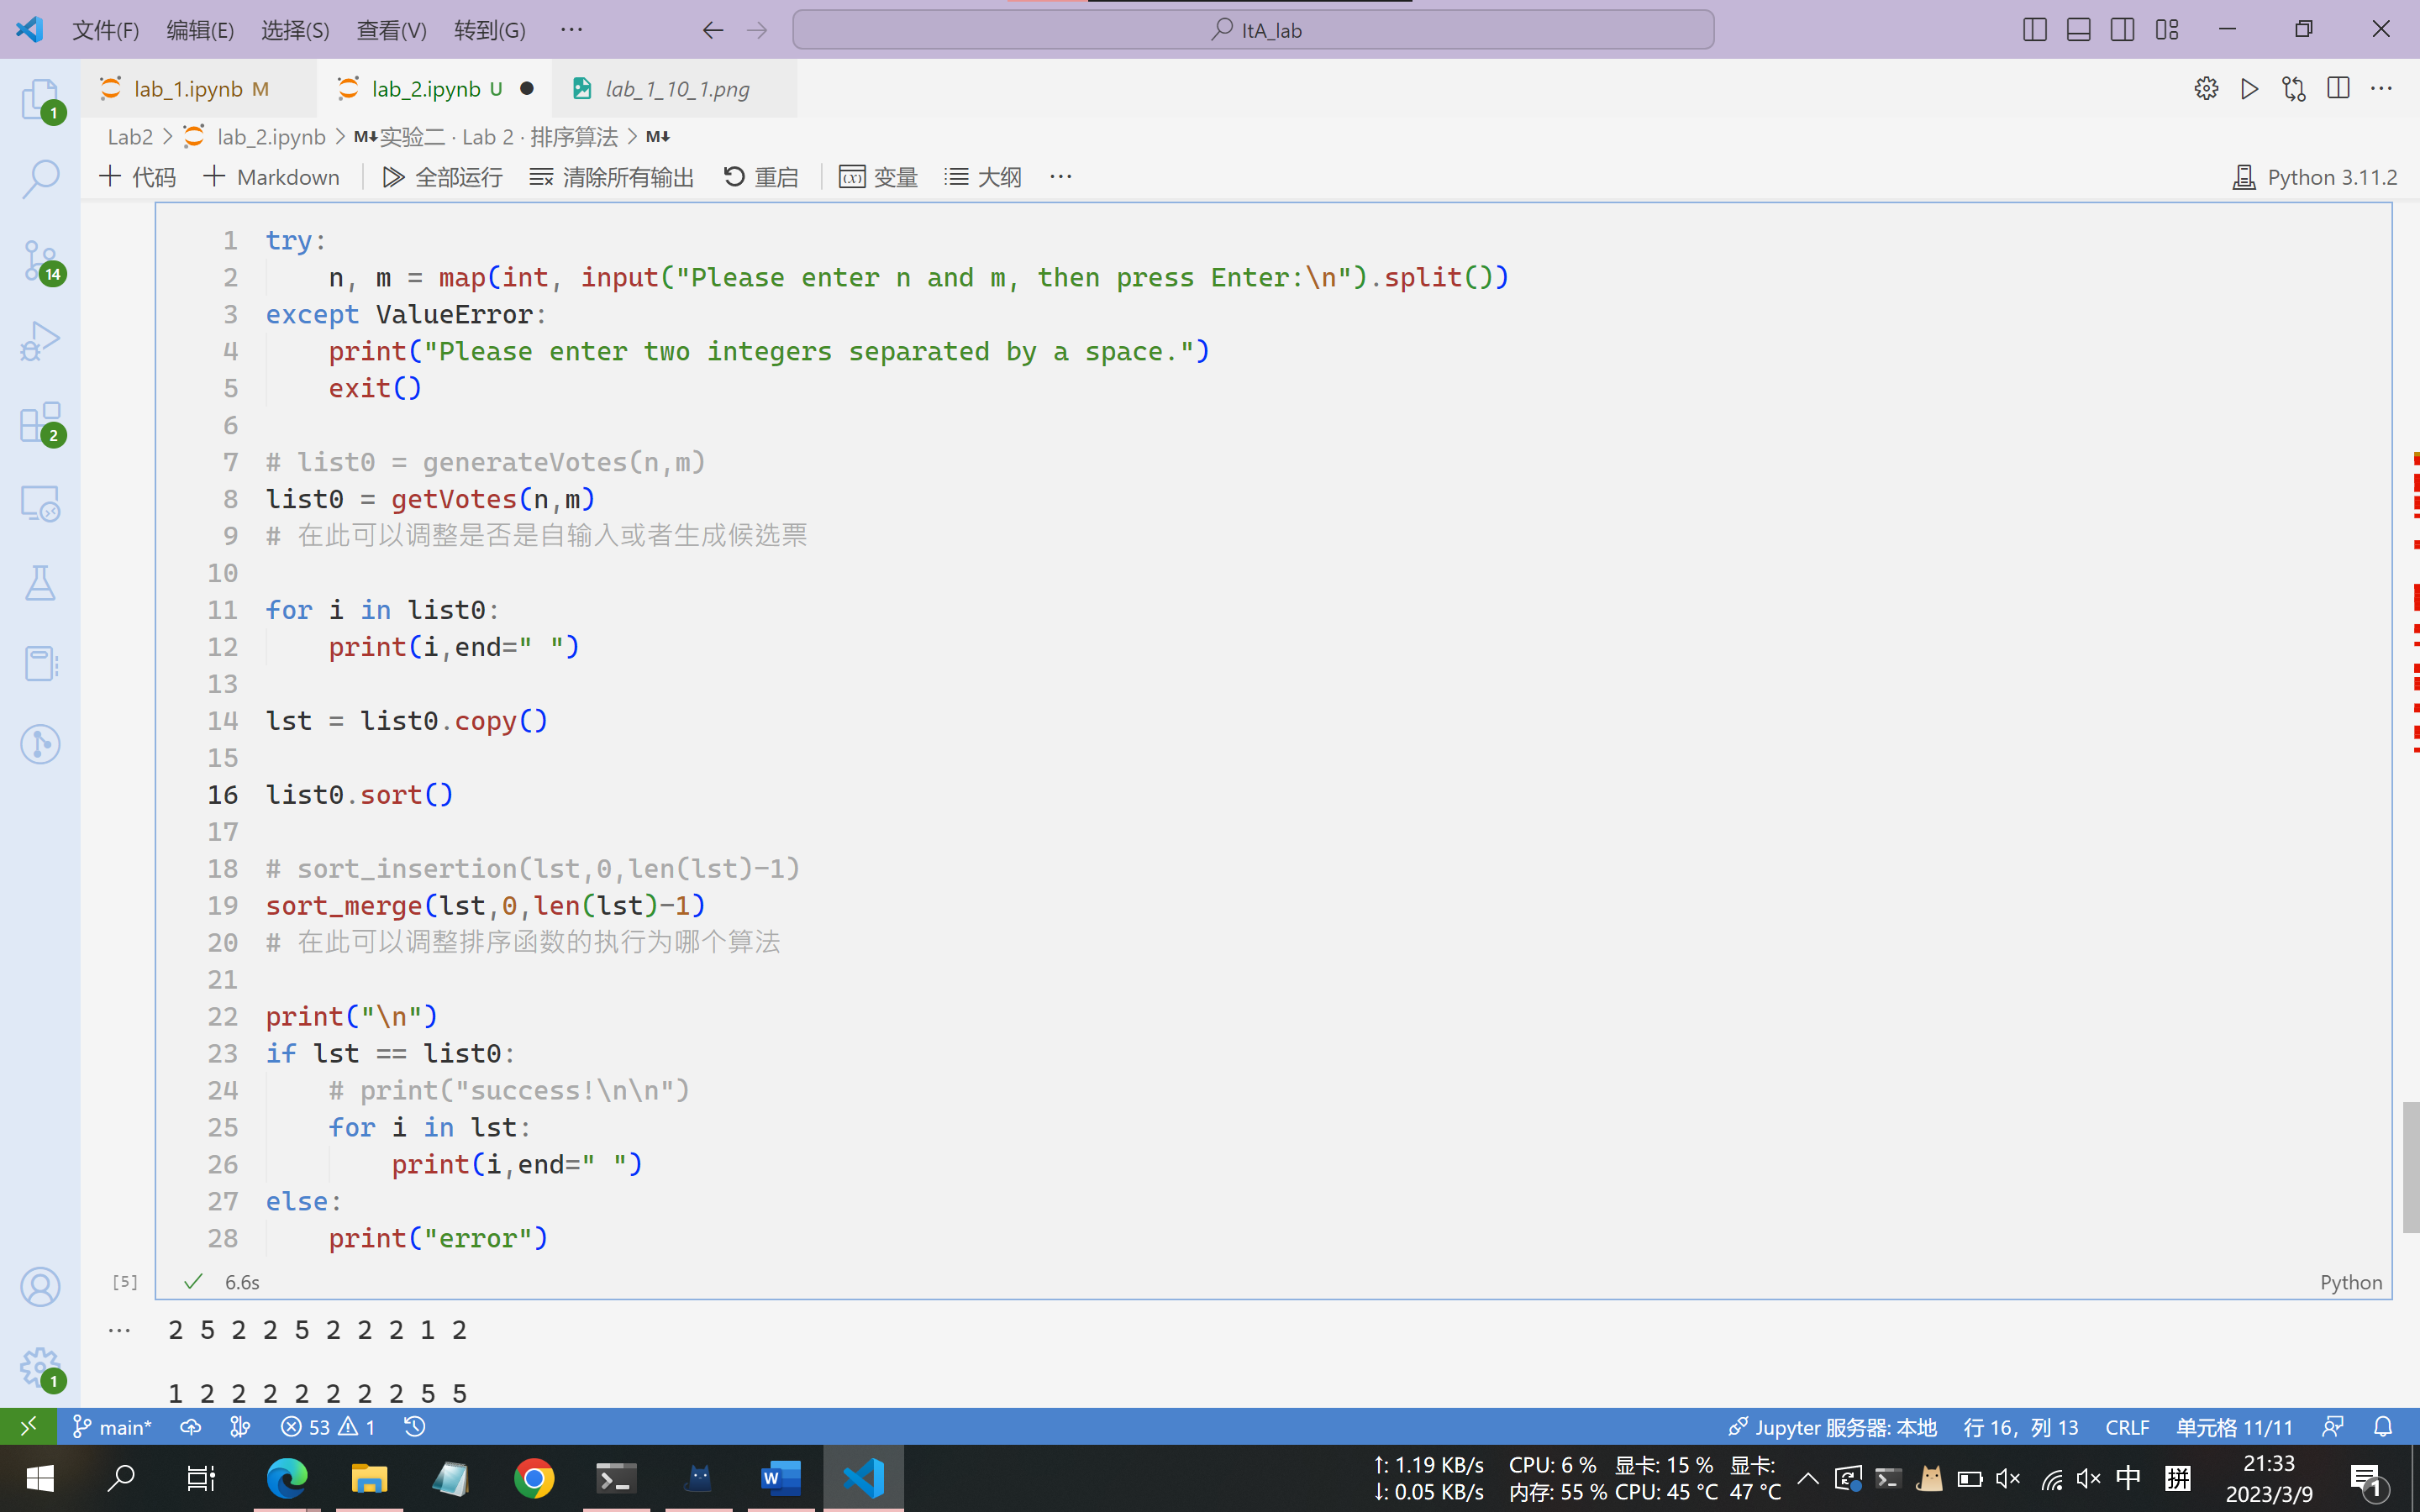
\includegraphics{./img/1.png}
\caption{如图所示}
\end{figure}

https://github.com/yuxiio/ItA\_lab.git 代码仓库地址

\hypertarget{ux603bux7ed3}{%
\subsection{总结}\label{ux603bux7ed3}}

设计算法问题时,应该考虑效率的同时,一定要保证可测试性和通用性。

因此我们可以设计一个通用测试框架,使用官方库运行出一个成功实例来对照。

当然本次实验中我也遇到了很多问题,比如python的变量实质其实就是名字标签加内存空间的绑定。因此list的复制和操作一定要注意。

同时我还遇到了TypeError: `list' object is not callable的错误。

通过debug我了解到了,在python中,尽量不要将变量命名为特定包的名字,不然变量名覆盖冲突会导致代码运行错误。
这是一个值得记住的编程经验。


    % Add a bibliography block to the postdoc
    
    
    
\end{document}
